\documentclass[12pt, twoside]{article}
\usepackage[letterpaper, margin=1in, head=30pt, headsep=0.1in]{geometry}
\usepackage[english]{babel}
\usepackage[utf8]{inputenc}
\usepackage{amsmath}
\usepackage{amsfonts}
\usepackage{amssymb}
\usepackage{tikz}
%\usetikzlibrary{quotes, angles}

\usepackage{graphicx}
\usepackage{enumitem}
\usepackage{multicol}

%\usepackage{pgfplots}
%\pgfplotsset{width=10cm,compat=1.9}
%\usepgfplotslibrary{statistics}
%\usepackage{pgfplotstable}
%\usepackage{tkz-fct}
%\usepackage{venndiagram}

\usepackage{fancyhdr}
\pagestyle{fancy}
\fancyhf{}
\renewcommand{\headrulewidth}{0pt} % disable the underline of the header
\raggedbottom
\newif\ifmeta
\metatrue %print standards and topics tags

\title{Math AI Worksheet Generator and Formative Assessment System}
\author{Chris Huson}
\date{August 2019}

\fancyhead[RE]{\thepage}
\fancyhead[RO]{\thepage \\ Name: \hspace{3cm}}
%\fancyhead[L]{BECA / Dr. Huson / 10th Grade Geometry\\* 7 June 2019}
%
%\begin{document}
%\subsubsection*{13.7 Homework: Cross sections, distance applications}
\fancyhead[L]{BECA / Dr. Huson / Geometry 04-Transversals\\* pset ID: 46}

\begin{document}

\subsubsection*{4-10PreExam-Transversals}
\begin{enumerate}
\item Construct a line perpendicular to $l$ though $C$.\\
    %\hspace{1cm} Given the line  $l$ and point $P$.
    \vspace{2cm}
    \begin{center}
    \begin{tikzpicture}
      \draw [<->, thick] (0,0)--(11,0) node[below left]{$l$};
      %\draw [fill] (0,0) circle [radius=0.05] node[left]{$A$};
      %\draw [fill] (11,0) circle [radius=0.05] ;
      \draw [fill] (7,2) circle [radius=0.05] node[above right]{$C$};
    \end{tikzpicture}
  \end{center} \vspace{2cm}

\item Complete the construction of the bisector of the given angle. 
  \vspace{2cm}
    \begin{center}
    \begin{tikzpicture}[rotate=20]
      \draw [<->, thick] (80:7)--(0,0)--(9,0);
      %\draw [fill] (0,0) circle [radius=0.05] node[below]{$A$};
      %\draw [fill] (5,0) circle [radius=0.05] node[below]{$B$};
    \end{tikzpicture}
    \end{center} \vspace{3cm}  

\newpage

\subsubsection*{Do Not Solve. Circle the appropriate equation and state the justification}
Use the postulates and theorems you have learned. You may abbreviate them as follows: ``def. of bisector," ``$\perp$ rays  with complementary $\angle$s adding to 90," ``linear pairs add to 180," ``vertical $\angle$s are $\cong$," ``corresponding $\angle$s of $\parallel$ lines are $\cong$," ``same-side interior $\angle$s are supplementary,'' ``alternate interior $\angle$s are $\cong$.''

\item Given $m \angle 1 = 4x+6$, $m \angle 2 = 6x-32$. Find $m \angle 1$.
  \hspace{2cm}
  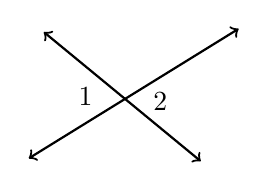
\begin{tikzpicture}[scale=.3, rotate=15]
    \draw [<->, thick] (0,-1.5)--(10,1.5);
    \draw [<->, thick] (2,3.5)--(7,-3.5);
    \node at (3,.4){1};
    \node at (6,-.6){2};
  \end{tikzpicture}\\[0.5cm]
  $\angle 1 \cong \angle 2$ \hspace{1cm} $m\angle 1 + m\angle 2 =  180$ \hspace{0.5cm} \rule{6cm}{0.15mm}
  \vspace{0.5cm}

\item Given two parallel lines and a transversal, as shown. \hspace{2cm}
  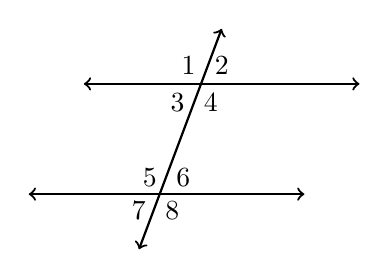
\begin{tikzpicture}[scale=0.7]
    \draw [<->, thick] (3,2)--(8,2);
    \draw [<->, thick] (2,0)--(7,0);
    \draw [<->, thick] (4,-1)--(5.5,3);
    \node at (4.5,0.3) [left]{$5$};
    \node at (4.5,0.3) [right]{$6$};
    \node at (4.3,-0.3) [left]{$7$};
    \node at (4.3,-0.3) [right]{$8$};
    \node at (5.2,2) [above left]{$1$};
    \node at (5.2,2) [above right]{$2$};
    \node at (5,2) [below left]{$3$};
    \node at (5,2) [below right]{$4$};
  \end{tikzpicture} \\[0.5cm]
  $\angle 4 \cong \angle 6$ \hspace{1cm} $m\angle 3 + m\angle 5 =  180$ \hspace{0.5cm} \rule{6cm}{0.15mm}

\item Given $m\angle R=m\angle U =65$, and $m\angle UST=130$. Find $m\angle RSU$.
    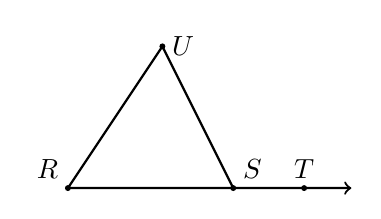
\begin{tikzpicture}[scale=0.6]
      %\draw [->, thick] (0,0)--(5,5);
      \draw [<-, thick] (7,0)--(1,0)--(3,3)--(4.5,0);
      \draw [fill] (1,0) circle [radius=0.05] node[above left]{$R$};
      \draw [fill] (4.5,0) circle [radius=0.05] node[above right]{$S$};
      \draw [fill] (3,3) circle [radius=0.05] node[right]{$U$};
      \draw [fill] (6,0) circle [radius=0.05] node[above]{$T$};
    \end{tikzpicture}\\[0.5cm]
    $\angle UST \cong \angle RSU$ \hspace{0.5cm} $m\angle UST + m\angle RSU =  180$ \hspace{0.5cm} \rule{6cm}{0.15mm} \vspace{0.25cm}

\item Given $\overrightarrow{BA} \perp \overrightarrow{BC}$, $m \angle ABD = 2x-5$, and $m \angle DBC = x-10$.
    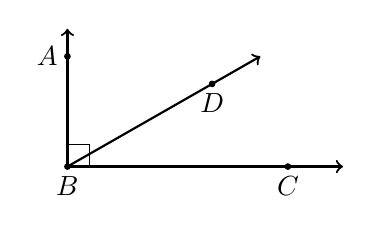
\begin{tikzpicture}[scale=0.7]
      \draw [<->, thick] (0,2.5)--(0,0)--(5,0);
      \draw [->, thick] (0,0)--(3.5, 2);
      \draw [-, thin] (0, 0.4)--(0.4, 0.4)--(0.4, 0);
      \draw [fill] (0,0) circle [radius=0.05] node[below]{$B$};
      \draw [fill] (0,2) circle [radius=0.05] node[left]{$A$};
      \draw [fill] (4,0) circle [radius=0.05] node[below]{$C$};
      \draw [fill] (2.625, 1.5) circle [radius=0.05] node[below]{$D$};
    \end{tikzpicture}\\[0.5cm]
    $\angle ABD \cong \angle DBC$ \hspace{0.5cm} $m\angle ABD + m\angle DBC =  90$ \hspace{0.5cm} \rule{6cm}{0.15mm}


\item $\overleftrightarrow{RPU}$ with ray $\overrightarrow{PS}$. \hspace{6cm}
    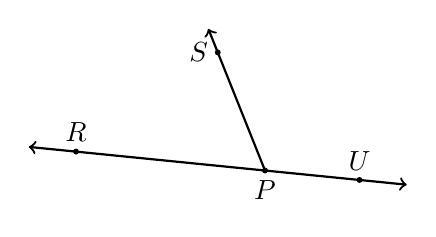
\begin{tikzpicture}[scale=0.6]
      \draw [<->, thick] (-5,.5)--(3,-.3);
      \draw [->, thick] (0,0)--(-1.2,3);
      \draw [fill] (-1,2.5) circle [radius=0.05] node[left ]{$S$};
      \draw [fill] (0,0) circle [radius=0.05] node[below]{$P$};
      \draw [fill] (2,-0.2) circle [radius=0.05] node[above]{$U$};
      \draw [fill] (-4,0.4) circle [radius=0.05] node[above]{$R$};
    \end{tikzpicture}\\[0.5cm]
    $\angle RPS \cong \angle SPU$ \hspace{0.25cm} $m \angle RPS + m \angle SPU = 180^\circ$ \hspace{0.25cm} \rule{6cm}{0.15mm}  \vspace{0.25cm}

\newpage
\item Find the sum of the measures of the internal angles of an octogon. Show the formula.  \vspace{4cm}

\item  A metal safety deposit box is $14 \frac{1}{2}$ inches long, 9 inches wide, and $2 \frac{1}{2}$ inches tall. Find the volume of the box. Show the calculation.
\begin{flushright}
  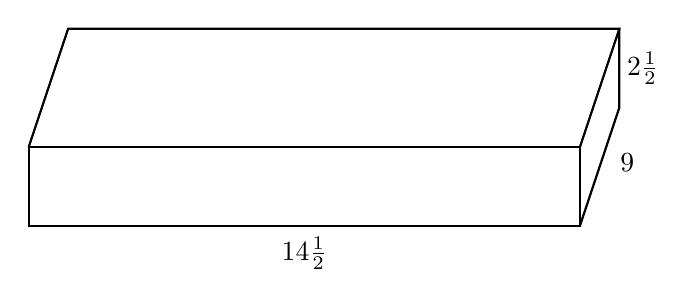
\begin{tikzpicture}[scale=1]
    \draw [-, thick] (0,0)--(7,0)--(7,1)--(0,1)--cycle;
    \draw [-, thick] (0,1)--(0.5,2.5)--(7.5,2.5)--(7,1);
    \draw [-, thick] (7,0)--(7.5,1.5)--(7.5,2.5);
    \node at (7.8, 2){$2 \frac{1}{2}$};
    \node at (3.5, -0.35){$14 \frac{1}{2}$};
    \node at (7.6, 0.8){$9$};
  \end{tikzpicture}
  \end{flushright} \vspace{2cm}


\item The circle $O$ is shown below with diameter $\overline{AOC}$ and radius $\overline{BO}$. Given $m\angle BAO = 73^\circ$. Find the measure of the central angle $\angle AOB$.
  \begin{flushright}
  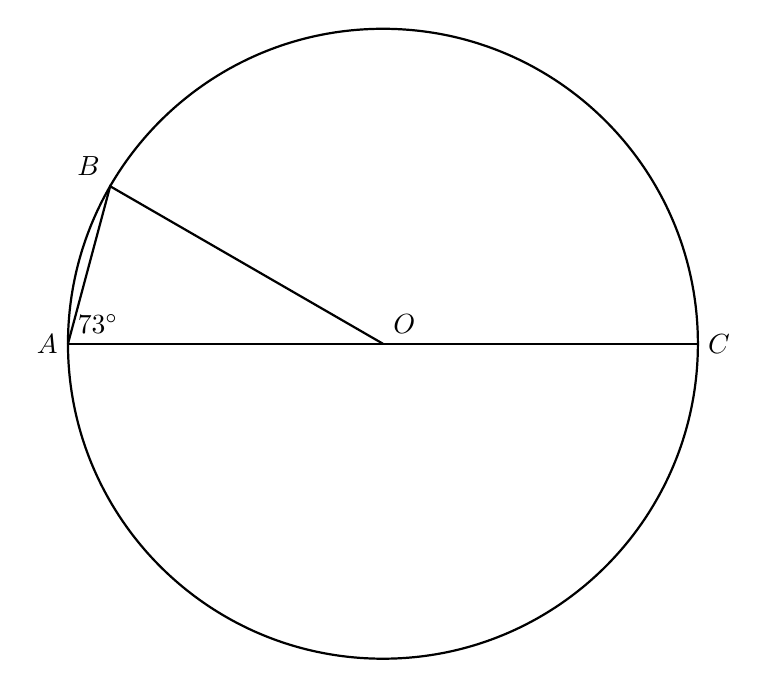
\begin{tikzpicture}[scale=0.8]
    \draw [thick] (0,0) circle [radius=5];
    \draw [-, thick] (-5,0) node[left]{$A$}--
    (0,0) node[above right]{$O$}--
    (5,0) node[right]{$C$};
    \draw [-, thick] (0,0)--(150:5) node[above left]{$B$}--(-5,0);
    \node at (-5, 0)[above right]{$73^\circ$};
  \end{tikzpicture}
  \end{flushright} \vspace{2cm}

\newpage
\item Given isosceles right $\triangle ABC$ with $\overline{AC} \cong \overline{BC}$ and $\overline{AC} \perp \overline{BC}$. Find $m\angle A$.
  \begin{flushright}
  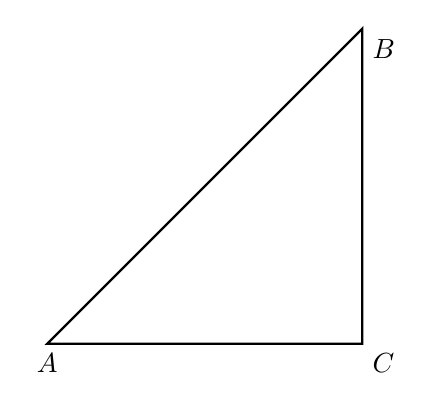
\begin{tikzpicture}[scale=0.5]
    \draw [thick](0,0) node[below]{$A$}--
    (8,0) node[below right]{$C$}--
    (8,8) node[below right]{$B$} --cycle;
  \end{tikzpicture}
  \end{flushright}  \vspace{0.5cm}
   
\item A sheet metal part is cut with square corners and two $45^\circ$ cutouts as shown with lengths marked in centimeters.
  \begin{enumerate}
    \item Find the area of the figure. (the drawing is not to scale)
      \begin{flushright}
      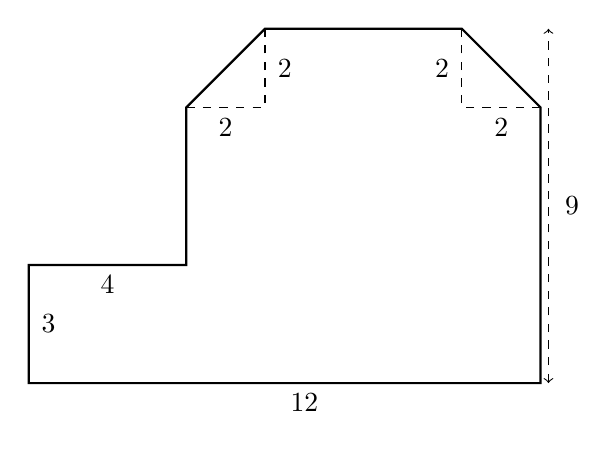
\begin{tikzpicture}[scale=0.5]
        \draw [-, thick] (0,0)--(13,0)--(13,7)--(11,9)--
        (6,9)--(4,7)--(4,3)--(0,3)--cycle;
        \draw [dashed] (4,7)--(6,7)--(6,9);
        \draw [dashed] (13,7)--(11,7)--(11,9);
        \draw [<->, dashed] (13.2,0)--(13.2,9);
        \node at (6.5, 8){2};
        \node at (5, 6.5){2};
        \node at (0.5, 1.5){3};
        \node at (2, 2.5){4};
        \node at (10.5, 8){2};
        \node at (12, 6.5){2};
        \node at (7, -0.5){12};
        \node at (13.8, 4.5){9};
        %\node at (13.5, 8){2};
      \end{tikzpicture}
      \end{flushright} \vspace{3cm}
    \item Spicy: The weight of the sheet metal is 1.5 grams per square centimeter. Find the weight of the part.
  \end{enumerate}

\newpage 

\item The measures in degrees of the three angles of a triangle are $3x$, $\frac{1}{2}x+7$, and $5x-65$. Find $x$. \vspace{4cm}

\item Given isosceles $\triangle RSU$ with $\overline{UR} \cong \overline{US}$. If $m\angle UST=x$ and $m\angle R=x-80$, find $m\angle U$.
  \begin{flushright}
  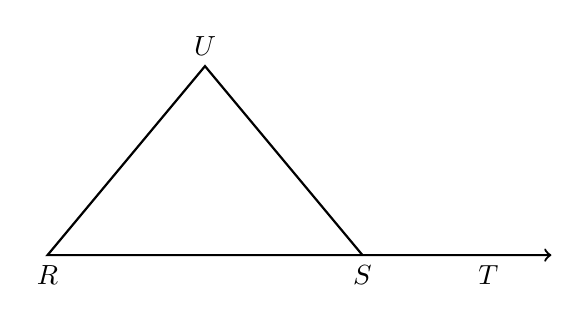
\begin{tikzpicture}[scale=0.8]
    %\draw [->, thick] (0,0)--(5,5);
    \draw [<-, thick] (8,0)--
      (7,0) node[below]{$T$}--
      (0,0) node[below]{$R$}--
      (2.5,3) node[above]{$U$}--
      (5,0) node[below]{$S$};
  \end{tikzpicture}
  \end{flushright} \vspace{2cm}
  
\item An angle bisector is shown below, with $\overrightarrow{AC}$ bisecting $\angle BAD$. Given $m\angle BAC = 3x+5$ and $m\angle BAD = 7x-1$, find $m\angle BAD$. (Show check)
  \begin{flushright}
  \begin{tikzpicture}[scale=0.7, rotate=20]
    \draw [<->, thick] (80:7)node[left]{$B$} 
    --(0,0)node[below]{$A$}
    --(6,0)node[below]{$D$}--(7,0);
    \draw [->, thick] (0,0)--(40:7)node[below right]{$C$};
    %\draw [fill] (0,0) circle [radius=0.05] node[below]{$A$};
    %\draw [fill] (5,0) circle [radius=0.05] node[below]{$B$};
  \end{tikzpicture}
  \end{flushright} \vspace{2cm}

\newpage


\item The trapezoid $ABCD$ has two parallel sides, $\overline{AB} \parallel \overline{CD}$ with lengths $AB=8$ and $CD=11$. The trapezoid's height is $h=6.5$. Find the areas of $\triangle ABC$ and $\triangle CDA$. Add their areas to find the area of the whole trapezoid. \\[0.25cm]
    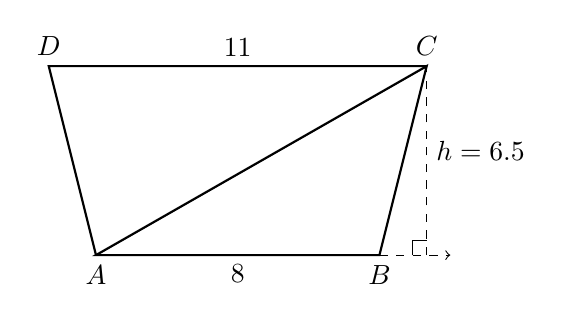
\begin{tikzpicture}[scale=0.6]
      \draw [thick]
        (0,0)node[below]{$A$}--
        (6,0)node[below]{$B$}--
        (7,4)node[above]{$C$} --cycle;
      \draw [thick] (0,0)--(-1,4)node[above]{$D$}--(7,4);
      \draw [dashed] (7,0)--(7,4);
      \draw [dashed, ->] (6,0)--(7.5,0);
      \draw (7,0)++(-0.3,0)--++(0,0.3)--+(0.3,0);
      \node at (7,2.2)[right]{$h=6.5$};
      \node at (3,0)[below]{$8$};
      \node at (3,4)[above]{$11$};
    \end{tikzpicture} \vspace{2cm}

\item Given parallel lines $\overleftrightarrow{AB} \parallel \overleftrightarrow{CDE}$ with $\overline{AC} \cong \overline{CD}$. If $m\angle BAD=80$ find $m\angle ACD$.
  \begin{flushright}
  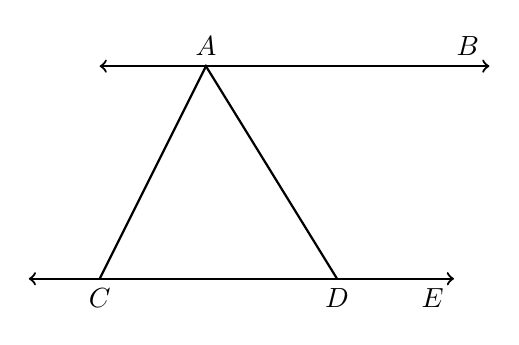
\begin{tikzpicture}[scale=0.9]
    \draw [<->, thick] (1,3)--(6.5,3) node[above left]{$B$};
    \draw [<->, thick] (0,0)--
      (5,0)--
      (6,0) node[below left]{$E$};
    \draw [-, thick] (1,0) node[below]{$C$}--
      (2.5,3) node[above]{$A$}--
      (4.35,0) node[below]{$D$};
  \end{tikzpicture}
  \end{flushright} \vspace{1cm}

\item Two parallel lines intersect a second set of parallel lines. Given $m\angle 2 = 2.8x+9$ and $m\angle 4 = 4.4x - 63$, find the measure of $\angle 1$. 
    \begin{flushright}
      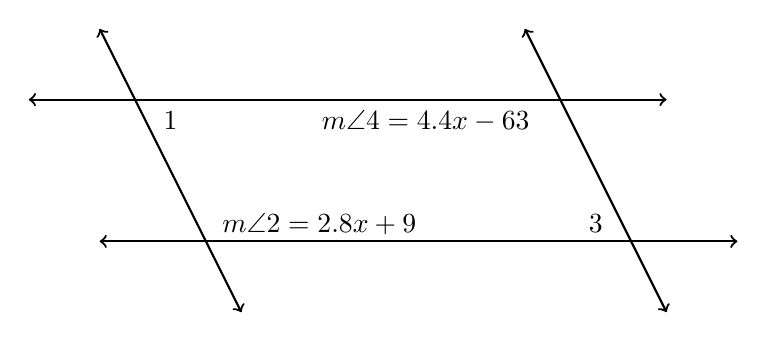
\begin{tikzpicture}[scale=0.9]
        \draw [<->, thick] (3,0)--(12,0);
        \draw [<->, thick] (2,2)--(11,2);
        \draw [<->, thick] (5,-1)--(3,3);
        \draw [<->, thick] (11,-1)--(9,3);
        \node at (4, 1.7){$1$};
        \node at (6.1, 0.25){$m\angle 2 = 2.8x+9$};
        \node at (10, 0.25){$3$};
        \node at (7.6, 1.7){$m\angle 4 = 4.4x - 63$};
      \end{tikzpicture}
      \end{flushright}

\newpage

    \subsubsection*{Do Not Solve! \\
    Label the drawing completely and write an equation in terms of $x$ modeling the situation.}
    \vspace{0.5cm}
  
\item Given that $O$ bisects $\overline{NP}$. $NO=2x$, $NP=3x+10$. Find ${x}$. \vspace{1cm}
  \begin{flushright}
    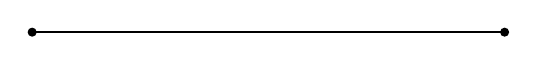
\begin{tikzpicture}
      \draw [-, thick] (0,0)--(6,0);
      \draw [fill] (0,0) circle [radius=0.05];
      \draw [fill] (6,0) circle [radius=0.05];
    \end{tikzpicture}
    \end{flushright} \vspace{2cm}
    
\item Given $\overline{ABC}$, with $AB=x-1$, $BC=3x+3$, and $AC=26$. Find ${AB}$. \vspace{1cm}
  \begin{flushright}
    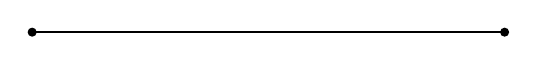
\begin{tikzpicture}
      \draw [-, thick] (0,0)--(6,0);
      \draw [fill] (0,0) circle [radius=0.05];
      \draw [fill] (6,0) circle [radius=0.05];
    \end{tikzpicture}
    \end{flushright} \vspace{2cm}
  
\item The points $R$, $S$, and $T$ are collinear, with $RS=3x-2$ and $ST=12$. If $RT=7x$, find ${RT}$. \vspace{1cm}
  \begin{flushright}
    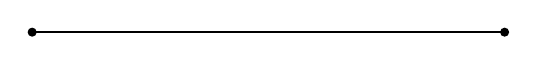
\begin{tikzpicture}
      \draw [-, thick] (0,0)--(6,0);
      \draw [fill] (0,0) circle [radius=0.05];
      \draw [fill] (6,0) circle [radius=0.05];
    \end{tikzpicture}
    \end{flushright} \vspace{2cm}
    
\item The point $K$ is the midpoint of $\overline{JL}$, $JK=10x+15$, and $JL=18x+40$. Find ${JK}$.  \vspace{1cm}
  \begin{flushright}
    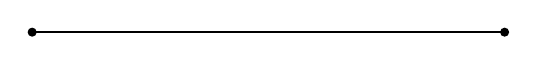
\begin{tikzpicture}
      \draw [-, thick] (0,0)--(6,0);
      \draw [fill] (0,0) circle [radius=0.05];
      \draw [fill] (6,0) circle [radius=0.05];
    \end{tikzpicture}
    \end{flushright} \vspace{2cm}

\newpage

\item Find the area of $\triangle CAT$. The altitude $h$ of the triangle is 6.7 centimeters and the base $CA=13.1$ cm. Show work by writing an equation before making the calculation. \\[0.5cm]
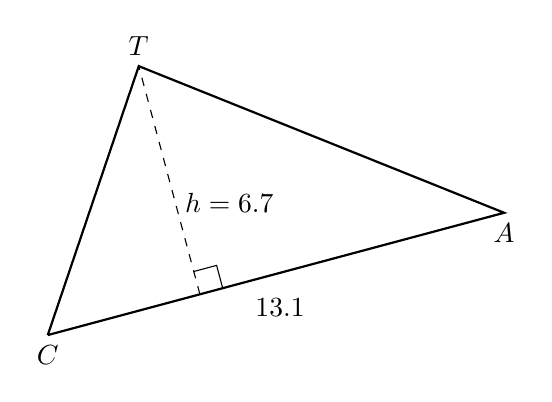
\begin{tikzpicture}[scale=1, rotate=15]
  \draw [thick]
    (2,0)node[below]{$C$}--
    (8,0)node[below]{$A$}--
    (4,3)node[above]{$T$} --(2,0);
 \draw [dashed] (4,0)--(4,3);
 \draw (4,0)++(0.3,0)--++(0,0.3)--+(-0.3,0);
 \node at (4,1.2)[right]{$h=6.7$};
 \node at (5,-0.2)[below]{$13.1$};
\end{tikzpicture} \vspace{1.0cm}


\item Given $\overleftrightarrow{RS}$ as shown on the number line, with $R=-3.1$ and $S=3.9$. \\[20pt] % Midpoint
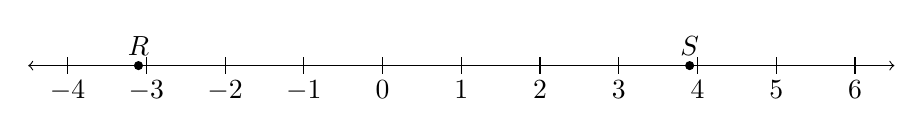
\begin{tikzpicture}
  \draw [<->] (-4.5,0)--(6.5,0);
  \foreach \x in {-4,...,6} %2 leading for diff!=1
    \draw[shift={(\x,0)},color=black] (0pt,-3pt) -- (0pt,3pt) node[below=5pt]  {$\x$};
    \draw [fill] (-3.1,0) circle [radius=0.05] node[above] {$R$};
    \draw [fill] (3.9,0) circle [radius=0.05] node[above] {$S$};
\end{tikzpicture}
\begin{enumerate}
  \item What is the exact distance on the number line between the points $R$ and $S$? \vspace{2cm} 
  \item The point $T$ bisects $\overline{RS}$. Find the value of $T$, and mark and label it on the numberline $\overleftrightarrow{RS}$ shown above. 
\end{enumerate} \vspace{2cm} 


\item Find the area of the parallelogram $ABCD$ shown below, with $AB=21.2$ and height $h=15.0$.
\begin{flushright}
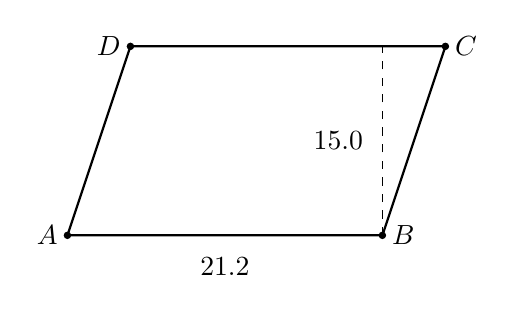
\begin{tikzpicture}[scale=0.8]
  \draw [-, thick] (0,0)--(5,0)--(6,3)--(1,3)--cycle;
  \draw [-, dashed] (5,0)--(5,3);
  \draw [fill] (0,0) circle [radius=0.05] node[left]{$A$};
  \draw [fill] (5,0) circle [radius=0.05] node[right]{$B$};
  \draw [fill] (6,3) circle [radius=0.05] node[right]{$C$};
  \draw [fill] (1,3) circle [radius=0.05] node[left]{$D$};
  \node at (4.3, 1.5){$15.0$};
  \node at (2.5, -0.5){21.2};
\end{tikzpicture}
\end{flushright}


\newpage
  \subsubsection*{Do Not Solve! \\
  Model the situation with an equation in terms of $x$. State whether the angles are complementary, supplementary, or vertical angles.}

\item Two lines intersect making four angles: $\angle 1$, $\angle 2$, $\angle 3$, and $\angle 4$. Given that $m\angle 3= 2x+50$ and $m\angle 4=6x+50$, find $x$.
  \begin{flushright}
  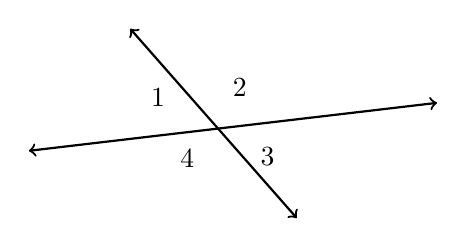
\begin{tikzpicture}[scale=0.5, rotate=-10]
  \draw [<->, thick] (0,-1.5)--(10,1.5);
  \draw [<->, thick] (2,2)--(7,-2);
  \node at (3,.4){1};
  \node at (6,-.6){3};
  \node at (5,1){2};
  \node at (4,-1){4};
  \end{tikzpicture}
  \end{flushright}

\item Given that $m\angle 1= 5x+22$ and $m\angle 3=7x+18$ as shown in the diagram, find $m\angle 2$.
  \begin{flushright}
  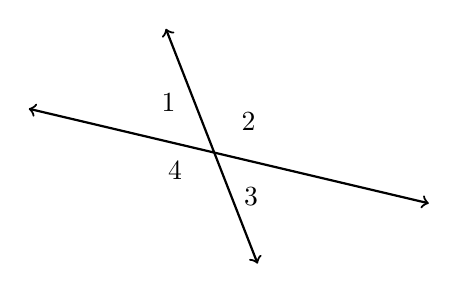
\begin{tikzpicture}[scale=0.5, rotate=-30]
  \draw [<->, thick] (0,-1.5)--(10,1.5);
  \draw [<->, thick] (2,2)--(7,-2);
  \node at (3,.4){1};
  \node at (6,-.6){3};
  \node at (5,1){2};
  \node at (4,-1){4};
  \end{tikzpicture}
  \end{flushright}

\item In the diagram below $m\angle AOB = 3x+5$ and $m\angle COB = 4x+15$. Find $x$. %\vspace{0.25cm}
  \begin{flushright}
  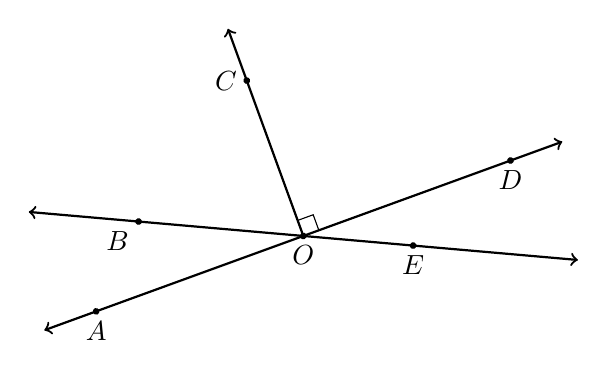
\begin{tikzpicture}[scale=0.7, rotate=20]
  \draw [<->, thick] (-25:5)--(0,0)--(155:5);
  \draw [<->, thick] (-5,0)--(5,0);
  \draw [->, thick] (0,0)--(0,4);
  \draw (0,0)++(0.3,0)--++(0,0.3)--+(-0.3,0);
  %\draw [fill] (-1,2.5) circle [radius=0.05] node[left ]{$B$};
  \draw [fill] (155:3) circle [radius=0.05] node[below left]{$B$};
  \draw [fill] (-4,0) circle [radius=0.05] node[below]{$A$}; 
  \draw [fill] (0,0) circle [radius=0.05] node[below]{$O$};
  \draw [fill] (0,3) circle [radius=0.05] node[left]{$C$};
  \draw [fill] (4,0) circle [radius=0.05] node[below]{$D$};
  \draw [fill] (-25:2) circle [radius=0.05] node[below]{$E$};
  \end{tikzpicture}
  \end{flushright}

\item In the diagram below $m\angle AOB = 65$, $m\angle BOC = 4x-10$, and $m\angle DOC = 3x+55^\circ$. Find $m\angle AOB$.
  \begin{flushright}
  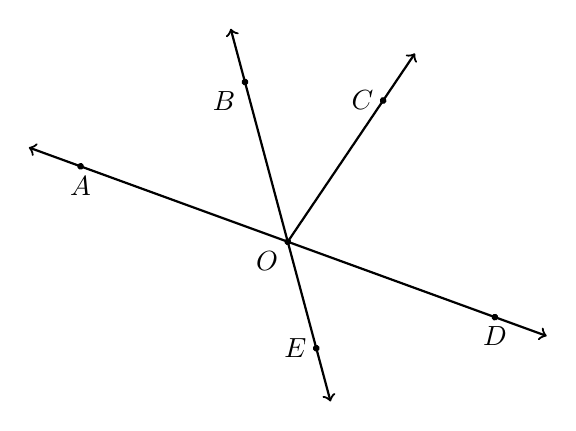
\begin{tikzpicture}[scale=0.7, rotate=-20]
  \draw [<->, thick] (-55:3)--(0,0)--(125:4);
  \draw [<->, thick] (-5,0)--(5,0);
  \draw [->, thick] (0,0)--(1,4);
  %\draw (0,0)++(0.3,0)--++(0,0.3)--+(-0.3,0);
  %\draw [fill] (-1,2.5) circle [radius=0.05] node[left ]{$B$};
  \draw [fill] (125:3) circle [radius=0.05] node[below left]{$B$};
  \draw [fill] (-4,0) circle [radius=0.05] node[below]{$A$}; 
  \draw [fill] (0,0) circle [radius=0.05] node[below left]{$O$};
  \draw [fill] (0.75,3) circle [radius=0.05] node[left]{$C$};
  \draw [fill] (4,0) circle [radius=0.05] node[below]{$D$};
  \draw [fill] (-55:2) circle [radius=0.05] node[left]{$E$};
  \end{tikzpicture}
  \end{flushright}

\newpage 

\item Complete the construction of an equilateral triangle with one side as $\overline{XY}$. Show all construction marks, but make no extra lines. \vspace{1cm}
  \begin{center}
  \begin{tikzpicture}[rotate=-20]
    \draw [-, thick] (0,0)--(0,5);
    \draw [fill] (0,0) circle [radius=0.05] node[below left]{$X$};
    \draw [fill] (0,5) circle [radius=0.05] node[above left]{$Y$};
  \end{tikzpicture}
  \end{center} \vspace{2cm}

\item Given the diagram shown below. \vspace{0.25cm}
  \begin{enumerate}
    \item  Measure the angle $AEB$. $m \angle AEB = $ \rule{4cm}{0.15mm} \bigskip
    \item Name an angle that is complementary to $\angle BEC$: \rule{4cm}{0.15mm} \bigskip
    \item Name a pair of opposite rays: \rule{4cm}{0.15mm}
  \end{enumerate}
  \vspace{1cm}
  \begin{center}
  \begin{tikzpicture}[scale=1.1, rotate=-30]
    \draw [->, thick] (0,0)--(55:5);
    \draw [<->, thick] (-5,0)--(6,0);
    \draw [->, thick] (0,0)--(0,3);
    \draw (0,0)++(0.3,0)--++(0,0.3)--+(-0.3,0);
    %\draw [fill] (-1,2.5) circle [radius=0.05] node[left ]{$B$};
    \draw [fill] (55:4) circle [radius=0.05] node[below right]{$B$};
    \draw [fill] (-4,0) circle [radius=0.05] node[below]{$A$};
    \draw [fill] (0,0) circle [radius=0.05] node[below left]{$E$};
    \draw [fill] (0,2) circle [radius=0.05] node[left]{$C$};
    \draw [fill] (4,0) circle [radius=0.05] node[below]{$D$};
  \end{tikzpicture}
  \end{center}

\newpage

\item One side of the $\triangle ABC$ has a length $AB=16$. The triangle's area is 96. Find the length of the altitude $h$ of the triangle to vertex $C$ and perpendicular to side $\overline{AB}$.\\[0.5cm]
  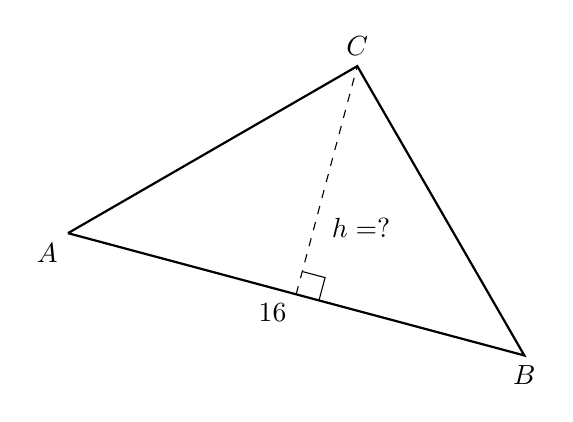
\begin{tikzpicture}[scale=1, rotate=-15]
  \draw [thick]
    (2,0)node[below left]{$A$}--
    (8,0)node[below]{$B$}--
    (5,3)node[above]{$C$} --(2,0);
  \draw [dashed] (5,0)--(5,3);
  \draw (5,0)++(0.3,0)--++(0,0.3)--+(-0.3,0);
  \node at (5.1,0.9)[right]{$h=?$};
  \node at (5,0)[below left]{$16$};
  \end{tikzpicture} \vspace{1.0cm}

\item The shape shown below is composed of straight lines and right angles, with some lengths as marked. Find the area of the figure. (the figure is not drawn to scale)
  \begin{flushleft}
  \begin{tikzpicture}[scale=0.5]
    \draw [-, thick] (0,0)--(13,0)--(13,3)--(9,3)--(9,9)--
    (0,9)--(0,7)--(4,7)--(4,3)--(0,3)--cycle;
    %\draw [fill] (0,0) circle [radius=0.05] node[left]{$A$};
    %\draw [fill] (7,0) circle [radius=0.05] node[right]{$B$};
    %\draw [fill] (7,2) circle [radius=0.05] node[right]{$C$};
    %\draw [fill] (0,2) circle [radius=0.05] node[left]{$D$};
    \node at (4.5, 5){3};
    \node at (2, 2.5){3};
    \node at (8.5, 5){5};
    \node at (11, 2.5){3};
    \node at (6.5, -0.5){10};
    \node at (13.5, 1.5){2};
    %\node at (13.5, 8){2};
  \end{tikzpicture}
  \end{flushleft} \vspace{2cm}

\item Given two complementary angles, $m\angle A = 54$ and $m\angle B = 3x-3$. Find $x$. Check your solution. \vspace{3.5cm} 

\item The volume of the rectanglar prism shown is 105 cubic meters. Its length is 7.5 meters and depth 4 m. Find its height $h$. Show the calculation. (not drawn to scale)
\begin{flushright}
  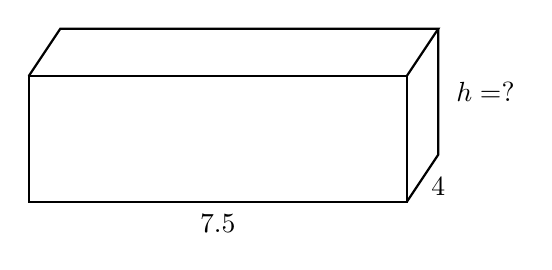
\begin{tikzpicture}[scale=0.8]
    \draw [-, thick] (0,0)--(6,0)--(6,2)--(0,2)--cycle;
    \draw [-, thick] (0,2)--(0.5,2.75)--(6.5,2.75)--(6,2);
    \draw [-, thick] (6,0)--(6.5,0.75)--(6.5,2.75);
    \node at (7.25, 1.75){$h=?$};
    \node at (3, -0.35){$7.5$};
    \node at (6.5, 0.25){$4$};
  \end{tikzpicture}
  \end{flushright} \vspace{1cm} 

\newpage

\subsubsection*{Complete all steps for full credit: the drawing to the top right, an equation and solution for $x$ on the left, followed by the answer to the question. Write the check to the bottom right.}

\item Given the collinear points $P$, $Q$, and $R$, with $PQ=7x+14$, $QR=2x+12$, and $PR=12x-10$. Find ${PQ}$.
  \vspace{9cm}

\item Angles $U$ and $V$ are supplementary. $m\angle U = 5x+61$ and $m\angle V = 3x-17$. Find $m\angle V$. \vspace{7cm}


\newpage
\subsubsection*{Early finishers, spicy}

\item The shape shown below is a trapezoid. Its height is 3.2 cm and the longer base is 6.0 cm. The shorter side opposite the base is 4.8 cm. \\[0.25cm]
  Find the area of the figure.
  \begin{flushright} 
  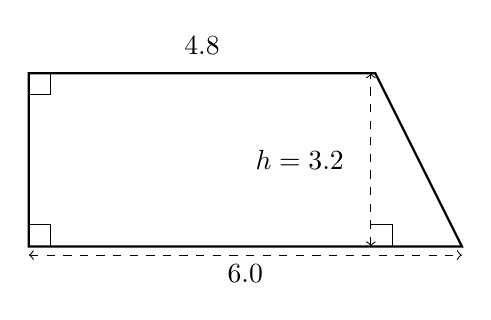
\begin{tikzpicture}[scale=1.1]
    \draw [thick]
    (3,0)--(3,2)--(7,2)--(8,0)--cycle;
    \draw [dashed,<->] (6.95,0)--(6.95,2);
    %\draw [dashed,<->] (0,2.1)--(7,2.1);
    %\draw [->] (45:0.5)--(45:0.9142);
    %\draw [->] (45:2.3)--(45:1.9142);
    \draw (3,0)++(0,0.25)--++(0.25,0)--+(0,-0.25);
    \draw (3,2)++(0,-0.25)--++(0.25,0)--+(0,0.25);
    \draw (6.95,0)++(0,0.25)--++(0.25,0)--+(0,-0.25);
    \draw [dashed,<->] (3,-0.1)--(8,-0.1);
    \node at (5.5,-0.1)[below]{$6.0$};
    \node at (6.75,1)[left]{$h=3.2$};
    \node at (5,2.1)[above]{$4.8$};
  \end{tikzpicture}
  \end{flushright} 
  \vspace{4cm}


\item In the diagram below $m\angle BOC = 3x+15$ and $m\angle DOE = 6x-6$. Find $m\angle DOE$.
  \begin{flushright}
  \begin{tikzpicture}[scale=0.8, rotate=-10]
    \draw [<->, thick] (-35:5)--(0,0)--(145:5);
    \draw [<->, thick] (-5,0)--(5,0);
    \draw [->, thick] (0,0)--(0,4);
    \draw (0,0)++(0.3,0)--++(0,0.3)--+(-0.3,0);
    %\draw [fill] (-1,2.5) circle [radius=0.05] node[left ]{$B$};
    \draw [fill] (145:3) circle [radius=0.05] node[below left]{$B$};
    \draw [fill] (-4,0) circle [radius=0.05] node[below]{$A$}; 
    \draw [fill] (0,0) circle [radius=0.05] node[below left]{$O$};
    \draw [fill] (0,3) circle [radius=0.05] node[left]{$C$};
    \draw [fill] (4,0) circle [radius=0.05] node[below]{$D$};
    \draw [fill] (-35:2) circle [radius=0.05] node[below left]{$E$};
  \end{tikzpicture}
  \end{flushright}


\newpage
\item An angle bisector is shown below, with $\overrightarrow{PR}$ bisecting $\angle QPS$. Given $m\angle QPR = 4x+2$ and $m\angle QPS = 10x-20$, find $m\angle QPS$.
  \begin{flushright}
  \begin{tikzpicture}[scale=0.6, rotate=30]
    \draw [<->, thick] (100:7)node[left]{$Q$} 
    --(0,0)node[below]{$P$}
    --(8,0)node[below]{$S$}--(9,0);
    \draw [->, thick] (0,0)--(50:7)node[below right]{$R$};
    %\draw [fill] (0,0) circle [radius=0.05] node[below]{$A$};
    %\draw [fill] (5,0) circle [radius=0.05] node[below]{$B$};
  \end{tikzpicture}
  \end{flushright} \vspace{4cm}
  
  \newpage

\item The length of the given rectangle is 10 more than the width. Its area is 75. Find the length and width of the rectangle using an algebraic method.\\[5pt]
  (the drawing is not to scale)
  \begin{flushright}
  \begin{tikzpicture}
    \draw [-, thick] (0,0)--(4.5,0)--(4.5,2)--(0,2)--cycle;
    \node at (5, 1){x};
    \node at (2.25, -0.5){$x+10$};
  \end{tikzpicture}
  \end{flushright} \vspace{5cm}

\item The circle with center $B$ is shown below with diameter $\overline{AC}$ and radius $\overline{BD}$. Given $AC=3x+15$ and $BD=2x+5$. Find the diameter of the circle.
  \begin{flushright}
  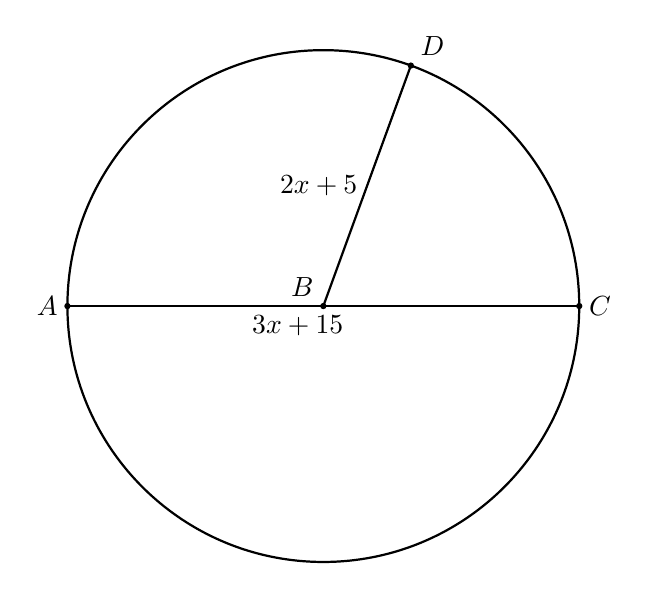
\begin{tikzpicture}[scale=0.65]
    \draw [thick] (0,0) circle [radius=5];
    \draw [-, thick] (-5,0)--(0,0)--(5,0);
    \draw [-, thick] (0,0)--(70:5);
    \draw [fill] (-5,0) circle [radius=0.05] node[left]{$A$};
    \draw [fill] (0,0) circle [radius=0.05] node[above left]{$B$};
    \draw [fill] (5,0) circle [radius=0.05] node[right]{$C$};
    \draw [fill] (70:5) circle [radius=0.05] node[above right]{$D$};
    \node at (70:2.5)[left]{$2x+5$};
    \node at (-0.5, 0)[below]{$3x+15$};
  \end{tikzpicture}
  \end{flushright} \vspace{2cm}

\newpage

\item Complete the construction of a hexagon with one side the given line segment. Show all construction marks, but make no extra lines. \vspace{9cm}
  \begin{center}
  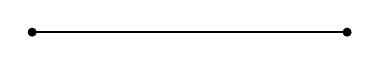
\begin{tikzpicture}
    \draw [-, thick] (0,0)--(4,0);
    \draw [fill] (0,0) circle [radius=0.05];
    \draw [fill] (4,0) circle [radius=0.05];
  \end{tikzpicture}
  \end{center} \vspace{4cm}

\item The area of a square is 20 cm. Find the perimeter of the square.

\end{enumerate}
\end{document}